\documentclass[12pt]{article}

%%%% Packages to be used
\usepackage{geometry}
\usepackage{graphicx}
% \graphicspath {{./../CleanSims/}}
\usepackage{amsmath, amssymb, amsfonts, amsthm, float}  
\usepackage{enumerate, color, framed, float, multirow}
\usepackage{comment, longtable, caption, subcaption, appendix}
\usepackage[sort,longnamesfirst]{natbib}
\usepackage{setspace, parskip}
\usepackage{placeins}

%%% Don't break up inline equations
% \binoppenalty=\maxdimen
% \relpenalty=\maxdimen


%%% Page Setup 
% \geometry{hmargin=3.5cm,vmargin={3cm,3cm},nohead,footskip=0.5in}
\renewcommand{\baselinestretch}{1.25}
\setlength{\baselineskip}{0.5in} \setlength{\parskip}{.05in}


\allowdisplaybreaks

%%% Table stretch
\renewcommand{\arraystretch}{1.2}
\setlength{\tabcolsep}{5pt}

%%% My Custom Commands
\newcommand{\pcite}[1]{\citeauthor{#1}'s \citeyearpar{#1}}

\newcommand{\ds}{\displaystyle}
\newcommand{\E}{\text{E}}
\newcommand{\Var}{\text{Var}}
\newcommand{\X}{\mathsf{X}}
\newcommand{\Y}{\mathsf{Y}}
\newcommand{\B}{\mathcal{B}}
\newcommand{\real}{{\mathbb R}}
\newcommand{\N}{{\mathbb N}}



\newcommand\numberthis{\addtocounter{equation}{1}\tag{\theequation}}

\newtheorem{theorem}{Theorem}
\newtheorem{defi}{Definition}
\newtheorem{propo}{Proposition}
\newtheorem{lemma}{Lemma}
\newtheorem{corollary}{Corollary}


\theoremstyle{remark}
\newtheorem{cond}{Condition}
\newtheorem{remark}{Remark}
\newtheorem{assum}{Assumption}
\newtheorem{example}{Example}



\begin{document}
\title{Revisiting the Gelman-Rubin Diagnostic}
\date{\today}
\author{Christina Knudson}
\maketitle


\section{Introduction} % (fold)
\label{sec:introduction}

The Gelman-Rubin (GR) diagnostic has been one of the most popular diagnostics for MCMC convergence. The GR diagnostic framework relies on  $m$  parallel chains ($m \geq 1$), each run for $n$ steps. The GR statistic (denoted $\hat{R}$) is the square root of the ratio of two estimators for the target variance.  In finite samples, the numerator overestimates this variance and the denominator underestimates it. Each estimator converges to the target variance, meaning that $\hat{R}$ converges to 1 as $n$ increases. When $\hat{R}$ becomes sufficiently close to 1, the GR diagnostic declares convergence. 





% section motivating_example (end)







\section{\textbf{Package building}}
\textbf{To do:}
\begin{itemize}
 \renewcommand{\labelitemi}{$\square$}
\item Clean up documentation
\item[$\blacksquare$] Add an example to \texttt{stable.gr} 
\item Check citations
\item Check descriptions and theory
\item Read through manual (pdf version)
\end{itemize}


\section{Effective sample size: \checkmark} % (fold)
\label{sec:choosing_delta}

For an estimator, effective sample size (ESS) is the number of independent samples with the same standard error as a correlated sample. 

\subsection{\texttt{n.eff} version 1.0}

The following is an expression for the lugsail-based psrf $\hat{R}^p_L$ for $m$  chains, each of length $n$ with  p components.
\begin{align*}
	\hat{R}^p_L &= \sqrt{ \left(\dfrac{n-1}{n} \right) + \dfrac{m}{\widehat{\text{ESS}}_L}},
\end{align*}
Rearranging this yields an estimator of effective sample size:
\begin{align*}
\widehat{\text{ESS}}_L = \dfrac{m}{\left( \hat{R}^p_L \right)^2 -  \left(\dfrac{n-1}{n} \right)}.
\end{align*}

\begin{remark}
	\label{rem:minimum_effort}
Vats et al (2018) explain that a minimum simulation effort must be set to safeguard from premature termination due to early bad estimates of $\sigma^2$. We concur and  suggest  a minimum simulation effort of $n = M_{\alpha, \epsilon,p}$. \\
\end{remark}

\textbf{Completed work} % (fold)


\begin{itemize}
 \renewcommand{\labelitemi}{$\square$}
\item[$\blacksquare$]  Added ESS calculation (now in \texttt{gr.diag} and \texttt{n.eff}).
\item[$\blacksquare$]  Added to \texttt{n.eff}. 
\begin{enumerate}
\item Called \texttt{target.psrf} using the info in their \texttt{mcmc.list} using  defaults.
\item Compared ESS to output of target.psrf and tell them whether this is sufficient for convergence.
\item If insufficient, calculate how many more samples needed using


\begin{align*}
\dfrac{n_\text{current}}{n_{ \text{current eff}}} \approx \dfrac{n_{\text{target}}}{n_{ \text{target eff}}}
\;\;\;  \Longrightarrow \;\;\;
 \dfrac{n_{\text{current}} \; n_{ \text{target eff}}}{n_{ \text{current eff}}}  \approx n_{\text{target}}.
\end{align*}
\item Added args of target.psrf.
\end{enumerate}
\end{itemize}

The way version 1.0 works: first ESS is calculated using the univariate psrf. Then, if the user says \texttt{multivariate = TRUE} and if \texttt{Nvar>1} (meaning it really is a multivariate chain), then we enter an \texttt{if} statement where a bunch of stuff is calculated (including a new mpsrf-based ESS, which then replaces the univariate psrf-based ESS).

\subsection{\texttt{n.eff} version 2.0} % (fold)
Version 2.0 of \texttt{n.eff} is all about NOT calling \texttt{gr.diag}, as that function performs calculations irrelevent to \texttt{n.eff}. Replacing version 1.0 with version 2.0 requires a bit of care: we want to use the univariate info in the univariate setting and the multivariate info in the multivariate setting.

Relevant univariate equation: \\

Relevant multivariate equation:

\begin{align*}
m n \left( \dfrac{\text{det}(\hat{S})}{\text{det}(\hat{T}_L)} \right)^{1/p}
\end{align*}

To create version 2.0 of \texttt{n.eff}, the following work must be done:

\begin{itemize}
 \renewcommand{\labelitemi}{$\square$}
\item[$\blacksquare$]   asymptotic variances
\begin{itemize}
\item write function \checkmark
\item documentation \checkmark
\item test \checkmark (tests stayed same before/after implementation)
\end{itemize}

\item[$\blacksquare$]   asymptotic variance matrix
\begin{itemize}
\item write function \checkmark
\item documentation \checkmark
\item test \checkmark (tests stayed same before/after implementation)
\end{itemize}

\item[$\blacksquare$]   sample variances s and variance matrix
\begin{itemize}
\item write function \checkmark
\item test \checkmark (tests stayed same before/after implementation)
\end{itemize}

\item[$\blacksquare$]  Rewrite \texttt{stable.GR} to call these functions



\item[$\blacksquare$] Rewrite \texttt{n.eff} to call these functions (rather than calling \texttt{stable.gr}).

%\item Figure out how to send some arguments from ellipsis of \texttt{n.eff} to \texttt{gr.diag} and others to \texttt{target.psrf}. 
\item[$\blacksquare$] Add an example.

\end{itemize}





\section{\textbf{Moving away from coda \checkmark}}

Due to known coding errors (e.g. the miscalculated confidence interval for $\hat{R}$) and issues with \texttt{coda}, we would like to change our package (functions including \texttt{n.eff} and \texttt{gr.diag}) to no longer rely on \texttt{coda}. An incomplete list of ways we rely on  \texttt{coda}: 

\begin{itemize}
 \renewcommand{\labelitemi}{$\blacksquare$}
\item Users are required to input an \texttt{mcmc.list} in our current version. We should replace this with a list such that each object in the list is a matrix representing a single Markov chain: each row is one iteration and each column is one variable)
\item An \texttt{mcmclist} has \texttt{mcmc} objects. We will replace each mcmc object with a matrix (as described in the previous bullet). We need to keep in mind that \texttt{mcmc} performs several input checks, so we will need to perform our own checks. For example, we will need to check that all objects are of class matrix, and that the dims of each object in the list are identical. 

\item Our code calls \texttt{niter} to find \texttt{n}; we can replace this with the number of rows in the first object of the list. I choose the first since all the objects should have the same dims so it wouldn't matter which we choose. We know we will have at least one Markov chain so we will have a first.
\item We call \texttt{nvar} to find \texttt{p}; we can replace this with the number of columns in the first object of the list. See note in previous bullet.
\item \texttt{varnames} is currently pointlessly called
\item \texttt{nchain} currently is used to determine the number of chains. This is easy enough to replace: just use \texttt{length} of the list.
\end{itemize}



\section{\textbf{Implementing replicated batch means}}

Consider the parameter $\tau^2_n = nVar(\bar{X}_{i\cdot})$. In our first pass at estimator $\tau^2_n$, we used the average of each chain's batch means variance estimates. Now, we are moving towards using replicated batch means: essentially, we will pool the chains together and use the floor of the square root of a \textit{single} chain's length (rather than the conglomerated Monte Carlo sample size.)  With the \texttt{mcmcse} function \texttt{mcse.mat}, it's easy to specify the batch size with the \texttt{size} argument.\\

We have to think a little more because \texttt{mcse.mat} (and \texttt{mcse.multi}) automate some things that we will now have to consider. In particular, \texttt{mcse.mat} (and \texttt{mcse.multi}) takes care of choosing which Monte Carlo samples to trim off in order to use the correct batch size. Now we will need to: 
\begin{enumerate}
\item Calculate the correct Monte Carlo batch size (floor of square root of a single chain's length).
\item Split each chain into batches by trimming the samples at the start of the chain rather than at the tail of the chain (see sketch below).
\item Stack the chains on top of each other (rbind).
\item Pass the conglomerated chain to mcse.mat (and also pass the correct batch size). 
\end{enumerate}

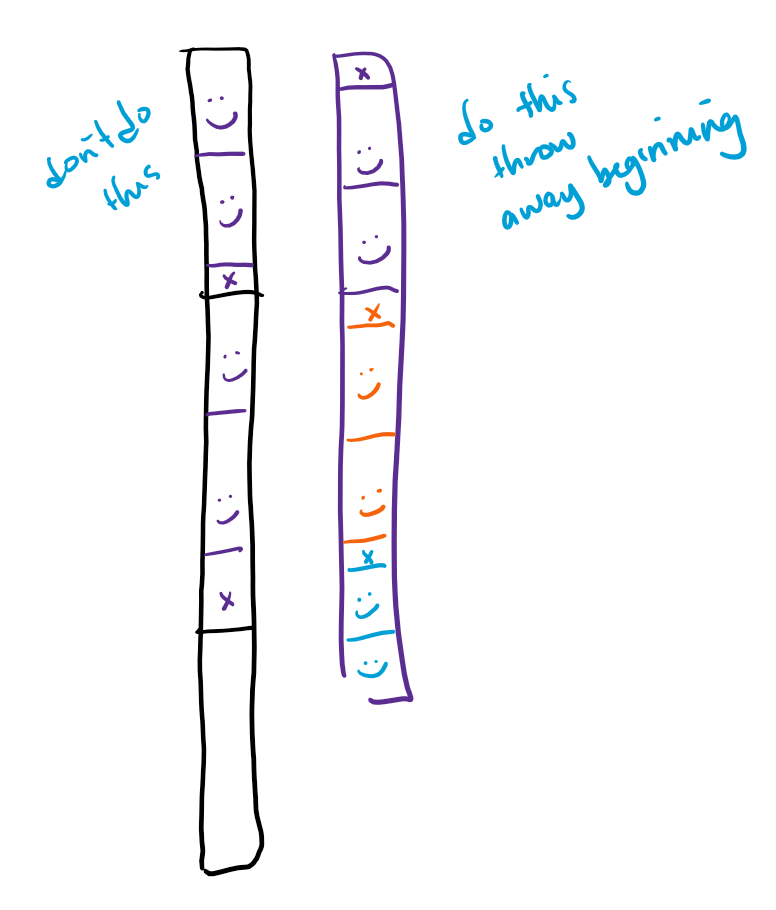
\includegraphics[width=3in]{repBMstackchains.png}\\

These calculations should be done in \texttt{asym.var}, since this function calls \texttt{mcse.mat} (and \texttt{mcse.multi}).
We  also need to implement replicated batch means for matrix T (the multivariate version of $\tau^2_n$),  which calls \texttt{mcse.multi} rather than \texttt{mcse.mat}.\\

To do list:

\begin{itemize} \renewcommand{\labelitemi}{$\square$}
\item Implement replicated batch means for the univariate PSRF
\item Implemented replicated batch means for the MPSRF 
\end{itemize}


\bibliographystyle{apalike}
\bibliography{mcref}
\end{document}



